
                \documentclass[8pt]{beamer}
                \usepackage{beamerthemesplit}
                %\usepackage[orientation=portrait,size=custom,width=60,height=80, scale = 1.4]{beamerposter} 
                \geometry{papersize={16cm,22cm}}
                \usetheme{CambridgeUS} 
                \usepackage{textpos} 
                \usepackage[latin1]{inputenc} 
                \usepackage{amsmath} 
                \usepackage{mathtools} 
                \usepackage{color} 
                \usepackage{mathabx} 
                \usepackage{microtype} % Miglioramento dell'allineamento del testo
                \usepackage{ragged2e} % Miglioramento dell'allineamento del testo
                \usepackage{graphicx}
                \usepackage{longtable} 
                \usepackage{tikz} 
                \usepackage{esvect} 
                \usetikzlibrary{arrows,shapes} 
                \usecolortheme{beaver} 
                \usepackage{graphicx} 
                \usepackage{booktabs}
                \usepackage{changepage} 
                \setbeamertemplate{navigation symbols}{} 
                \setbeamertemplate{navigation symbols}{} 
            
        \title{GEANT4 Simulation Report}
        \author{Riccardo Nicolaidis \footnote{riccardo.nicolaidis@unitn.it}}
        \date{\today}
        
        \begin{document}
        
            \begin{frame}
                \titlepage
            \end{frame}
            
            \begin{frame}
                \frametitle{Info}
            
                \centering
                GDML File Name : \textbf{ LEM\_VetoChannel\_2-worldVOL\_B\_DummyMaterials\_Parsed.gdml}
                
                
                \vspace{2 cm}
                \textbf{NTuple Info}:
                \vspace{1 cm}
                
        \begin{itemize}
        
        \item Ntuple ID: 0 Ntuple Name: Edep
        
        \item Ntuple ID: 0 Ntuple Column ID: 0 Ntuple Column Name: RandEnergy
        
        \item Ntuple ID: 0 Ntuple Column ID: 1 Ntuple Column Name: Xgen
        
        \item Ntuple ID: 0 Ntuple Column ID: 2 Ntuple Column Name: Ygen
        
        \item Ntuple ID: 0 Ntuple Column ID: 3 Ntuple Column Name: Zgen
        
        \item Ntuple ID: 0 Ntuple Column ID: 4 Ntuple Column Name: pDirX
        
        \item Ntuple ID: 0 Ntuple Column ID: 5 Ntuple Column Name: pDirY
        
        \item Ntuple ID: 0 Ntuple Column ID: 6 Ntuple Column Name: pDirZ
        
        \item Ntuple ID: 0 Ntuple Column ID: 7 Ntuple Column Name: EventID
        
        \item Ntuple ID: 0 Ntuple Column ID: 8 Ntuple Column Name: JobNumber
        
        \item Ntuple ID: 0 Ntuple Column ID: 9 Ntuple Column Name: Ed\_LV\_AlBottom
        
        \item Ntuple ID: 0 Ntuple Column ID: 10 Ntuple Column Name: Ed\_LV\_SiliconDetector\_Thin\_0
        
        \item Ntuple ID: 0 Ntuple Column ID: 11 Ntuple Column Name: Ed\_LV\_BakeliteBoardBottom
        
        \item Ntuple ID: 0 Ntuple Column ID: 12 Ntuple Column Name: Ed\_LV\_BakeliteBoardCalo
        
        \item Ntuple ID: 0 Ntuple Column ID: 13 Ntuple Column Name: Ed\_LV\_Calo
        
        \item Ntuple ID: 0 Ntuple Column ID: 14 Ntuple Column Name: Ed\_LV\_PlasticVetoTop
        
        \item Ntuple ID: 0 Ntuple Column ID: 15 Ntuple Column Name: Ed\_LV\_SiliconDetector\_Thin\_2
        
        \item Ntuple ID: 0 Ntuple Column ID: 16 Ntuple Column Name: Ed\_LV\_AlFrame\_Thin\_1
        
        \item Ntuple ID: 0 Ntuple Column ID: 17 Ntuple Column Name: Ed\_LV\_AlFrame\_Thin\_2
        
        \item Ntuple ID: 0 Ntuple Column ID: 18 Ntuple Column Name: Ed\_LV\_SiliconDetector\_Thin\_1
        
        \item Ntuple ID: 0 Ntuple Column ID: 19 Ntuple Column Name: Ed\_LV\_SiliconDetector\_Thin\_3
        
        \item Ntuple ID: 0 Ntuple Column ID: 20 Ntuple Column Name: Ed\_LV\_AlFrame\_Thick\_4
        
        \item Ntuple ID: 0 Ntuple Column ID: 21 Ntuple Column Name: Ed\_LV\_AlFrame\_Thick\_2
        
        \item Ntuple ID: 0 Ntuple Column ID: 22 Ntuple Column Name: Ed\_LV\_AlFrame\_Thick\_1
        
        \item Ntuple ID: 0 Ntuple Column ID: 23 Ntuple Column Name: Ed\_LV\_SiliconDetector\_Thick\_2
        
        \item Ntuple ID: 0 Ntuple Column ID: 24 Ntuple Column Name: Ed\_LV\_BakeliteCable\_Thick\_3
        
        \item Ntuple ID: 0 Ntuple Column ID: 25 Ntuple Column Name: Ed\_LV\_BakeliteCable\_Thick\_0
        
        \item Ntuple ID: 0 Ntuple Column ID: 26 Ntuple Column Name: Ed\_LV\_SiliconDetector\_Thick\_4
        
        \item Ntuple ID: 0 Ntuple Column ID: 27 Ntuple Column Name: Ed\_LV\_AlScrew\_Thick\_2
        
        \item Ntuple ID: 0 Ntuple Column ID: 28 Ntuple Column Name: Ed\_LV\_SiliconDetector\_Thick\_1
        
        \item Ntuple ID: 0 Ntuple Column ID: 29 Ntuple Column Name: Ed\_LV\_AlScrew\_Thick\_1
        
        \item Ntuple ID: 0 Ntuple Column ID: 30 Ntuple Column Name: Ed\_LV\_AlScrew\_Thick\_4
        
        \item Ntuple ID: 0 Ntuple Column ID: 31 Ntuple Column Name: Ed\_LV\_SiliconDetector\_Thick\_0
        
        \item Ntuple ID: 0 Ntuple Column ID: 32 Ntuple Column Name: Ed\_LV\_BakeliteCable\_Thick\_4
        
        \item Ntuple ID: 0 Ntuple Column ID: 33 Ntuple Column Name: Ed\_LV\_BakeliteCable\_Thick\_1
        
        \item Ntuple ID: 0 Ntuple Column ID: 34 Ntuple Column Name: Ed\_LV\_AlCoverLower
        
        \item Ntuple ID: 0 Ntuple Column ID: 35 Ntuple Column Name: Ed\_LV\_BakeliteCable\_Thick\_2
        
        \item Ntuple ID: 0 Ntuple Column ID: 36 Ntuple Column Name: Ed\_LV\_AlFrame\_Thick\_0
        
        \item Ntuple ID: 0 Ntuple Column ID: 37 Ntuple Column Name: Ed\_LV\_AlScrew\_Thick\_3
        
        \item Ntuple ID: 0 Ntuple Column ID: 38 Ntuple Column Name: Ed\_LV\_AlScrew\_Thick\_0
        
        \item Ntuple ID: 0 Ntuple Column ID: 39 Ntuple Column Name: Ed\_LV\_SiliconDetector\_Thick\_3
        
        \item Ntuple ID: 0 Ntuple Column ID: 40 Ntuple Column Name: Ed\_LV\_AlFrame\_Thin\_3
        
        \item Ntuple ID: 0 Ntuple Column ID: 41 Ntuple Column Name: Ed\_LV\_AlScrew
        
        \item Ntuple ID: 0 Ntuple Column ID: 42 Ntuple Column Name: Ed\_LV\_AlTop
        
        \item Ntuple ID: 0 Ntuple Column ID: 43 Ntuple Column Name: Ed\_LV\_AlScrew\_3
        
        \item Ntuple ID: 0 Ntuple Column ID: 44 Ntuple Column Name: Ed\_LV\_AlScrew\_1
        
        \item Ntuple ID: 0 Ntuple Column ID: 45 Ntuple Column Name: Ed\_LV\_BakeliteBoardMiddleLower
        
        \item Ntuple ID: 0 Ntuple Column ID: 46 Ntuple Column Name: Ed\_LV\_BakeliteBoardMiddleUpper
        
        \item Ntuple ID: 0 Ntuple Column ID: 47 Ntuple Column Name: Ed\_LV\_AlScrew\_2
        
        \item Ntuple ID: 0 Ntuple Column ID: 48 Ntuple Column Name: Ed\_LV\_AlFrame\_Thick\_3
        
        \item Ntuple ID: 0 Ntuple Column ID: 49 Ntuple Column Name: Ed\_LV\_PlasticVetoBottom
        
        \item Ntuple ID: 0 Ntuple Column ID: 50 Ntuple Column Name: Ed\_LV\_AlCoverUpper
        
        \item Ntuple ID: 0 Ntuple Column ID: 51 Ntuple Column Name: Ed\_LV\_AlFrame\_Thin\_0
        
        \item Ntuple ID: 0 Ntuple Column ID: 52 Ntuple Column Name: Ed\_LV\_SiliconDetector\_Thin\_4
        
        \item Ntuple ID: 0 Ntuple Column ID: 53 Ntuple Column Name: Ed\_LV\_AlFrame\_Thin\_4
        
        \item Ntuple ID: 1 Ntuple Name: Hits
        
        \item Ntuple ID: 1 Ntuple Column ID: 0 Ntuple Column Name: X
        
        \item Ntuple ID: 1 Ntuple Column ID: 1 Ntuple Column Name: Y
        
        \item Ntuple ID: 1 Ntuple Column ID: 2 Ntuple Column Name: Z
        
        \item Ntuple ID: 1 Ntuple Column ID: 3 Ntuple Column Name: E
        
        \end{itemize}
        
            \end{frame}
            
            \begin{frame}
                \frametitle{Material Info}
            
            \begin{table}
            \begin{tabular}{lll}
             Volume & Material & Mass (g) \\
                    
            \midrule
            LV\_AlBottom & G4\_Galactic & 1.56411e-23\\
                        LV\_SiliconDetector\_Thin\_0 & G4\_Si & 0.0104495\\
                        LV\_BakeliteBoardBottom & G4\_Galactic & 1.52827e-24\\
                        LV\_BakeliteBoardCalo & G4\_Galactic & 6.12395e-25\\
                        LV\_Calo & G4\_PLASTIC\_SC\_VINYLTOLUENE & 74.304\\
                        LV\_PlasticVetoTop & G4\_PLASTIC\_SC\_VINYLTOLUENE & 253.088\\
                        LV\_SiliconDetector\_Thin\_2 & G4\_Si & 0.0325397\\
                        LV\_AlFrame\_Thin\_1 & G4\_Galactic & 8.49576e-26\\
                        LV\_AlFrame\_Thin\_2 & G4\_Galactic & 8.49576e-26\\
                        LV\_SiliconDetector\_Thin\_1 & G4\_Si & 0.0325397\\
                        LV\_SiliconDetector\_Thin\_3 & G4\_Si & 0.0325397\\
                        LV\_AlFrame\_Thick\_4 & G4\_Galactic & 1.10354e-25\\
                        LV\_AlFrame\_Thick\_2 & G4\_Galactic & 1.10354e-25\\
                        LV\_AlFrame\_Thick\_1 & G4\_Galactic & 1.10354e-25\\
                        LV\_SiliconDetector\_Thick\_2 & G4\_Si & 0.135903\\
                        LV\_BakeliteCable\_Thick\_3 & G4\_Galactic & 1.72314e-26\\
                        LV\_BakeliteCable\_Thick\_0 & G4\_Galactic & 1.65354e-26\\
                        LV\_SiliconDetector\_Thick\_4 & G4\_Si & 0.135903\\
                        LV\_AlScrew\_Thick\_2 & G4\_Galactic & 7.9467e-26\\
                        LV\_SiliconDetector\_Thick\_1 & G4\_Si & 0.135903\\
                        LV\_AlScrew\_Thick\_1 & G4\_Galactic & 7.9467e-26\\
                        LV\_AlScrew\_Thick\_4 & G4\_Galactic & 7.9467e-26\\
                        LV\_SiliconDetector\_Thick\_0 & G4\_Si & 0.0439621\\
                        LV\_BakeliteCable\_Thick\_4 & G4\_Galactic & 1.72314e-26\\
                        LV\_BakeliteCable\_Thick\_1 & G4\_Galactic & 1.72314e-26\\
                        LV\_AlCoverLower & G4\_Galactic & 8.88373e-25\\
                        LV\_BakeliteCable\_Thick\_2 & G4\_Galactic & 1.72314e-26\\
                        LV\_AlFrame\_Thick\_0 & G4\_Galactic & 8.11217e-26\\
                        LV\_AlScrew\_Thick\_3 & G4\_Galactic & 7.9467e-26\\
                        LV\_AlScrew\_Thick\_0 & G4\_Galactic & 4.64453e-26\\
                        LV\_SiliconDetector\_Thick\_3 & G4\_Si & 0.135903\\
                        LV\_AlFrame\_Thin\_3 & G4\_Galactic & 8.49576e-26\\
                        LV\_AlScrew & G4\_Galactic & 2.02193e-25\\
                        LV\_AlTop & G4\_Galactic & 1.97275e-23\\
                        LV\_AlScrew\_3 & G4\_Galactic & 2.02193e-25\\
                        LV\_AlScrew\_1 & G4\_Galactic & 2.02193e-25\\
                        LV\_BakeliteBoardMiddleLower & G4\_Galactic & 1.13478e-24\\
                        LV\_BakeliteBoardMiddleUpper & G4\_Galactic & 1.25307e-24\\
                        LV\_AlScrew\_2 & G4\_Galactic & 2.02193e-25\\
                        LV\_AlFrame\_Thick\_3 & G4\_Galactic & 1.10354e-25\\
                        LV\_PlasticVetoBottom & G4\_PLASTIC\_SC\_VINYLTOLUENE & 128.504\\
                        LV\_AlCoverUpper & G4\_Galactic & 7.77017e-25\\
                        LV\_AlFrame\_Thin\_0 & G4\_Galactic & 4.81911e-26\\
                        LV\_SiliconDetector\_Thin\_4 & G4\_Si & 0.0325397\\
                        LV\_AlFrame\_Thin\_4 & G4\_Galactic & 8.49576e-26\\
                        
            \bottomrule
            \end{tabular}
            \end{table}
            
            \end{frame}
            
            \begin{frame}
                \frametitle{PID}
            
        \begin{figure}[h]
            \centering
            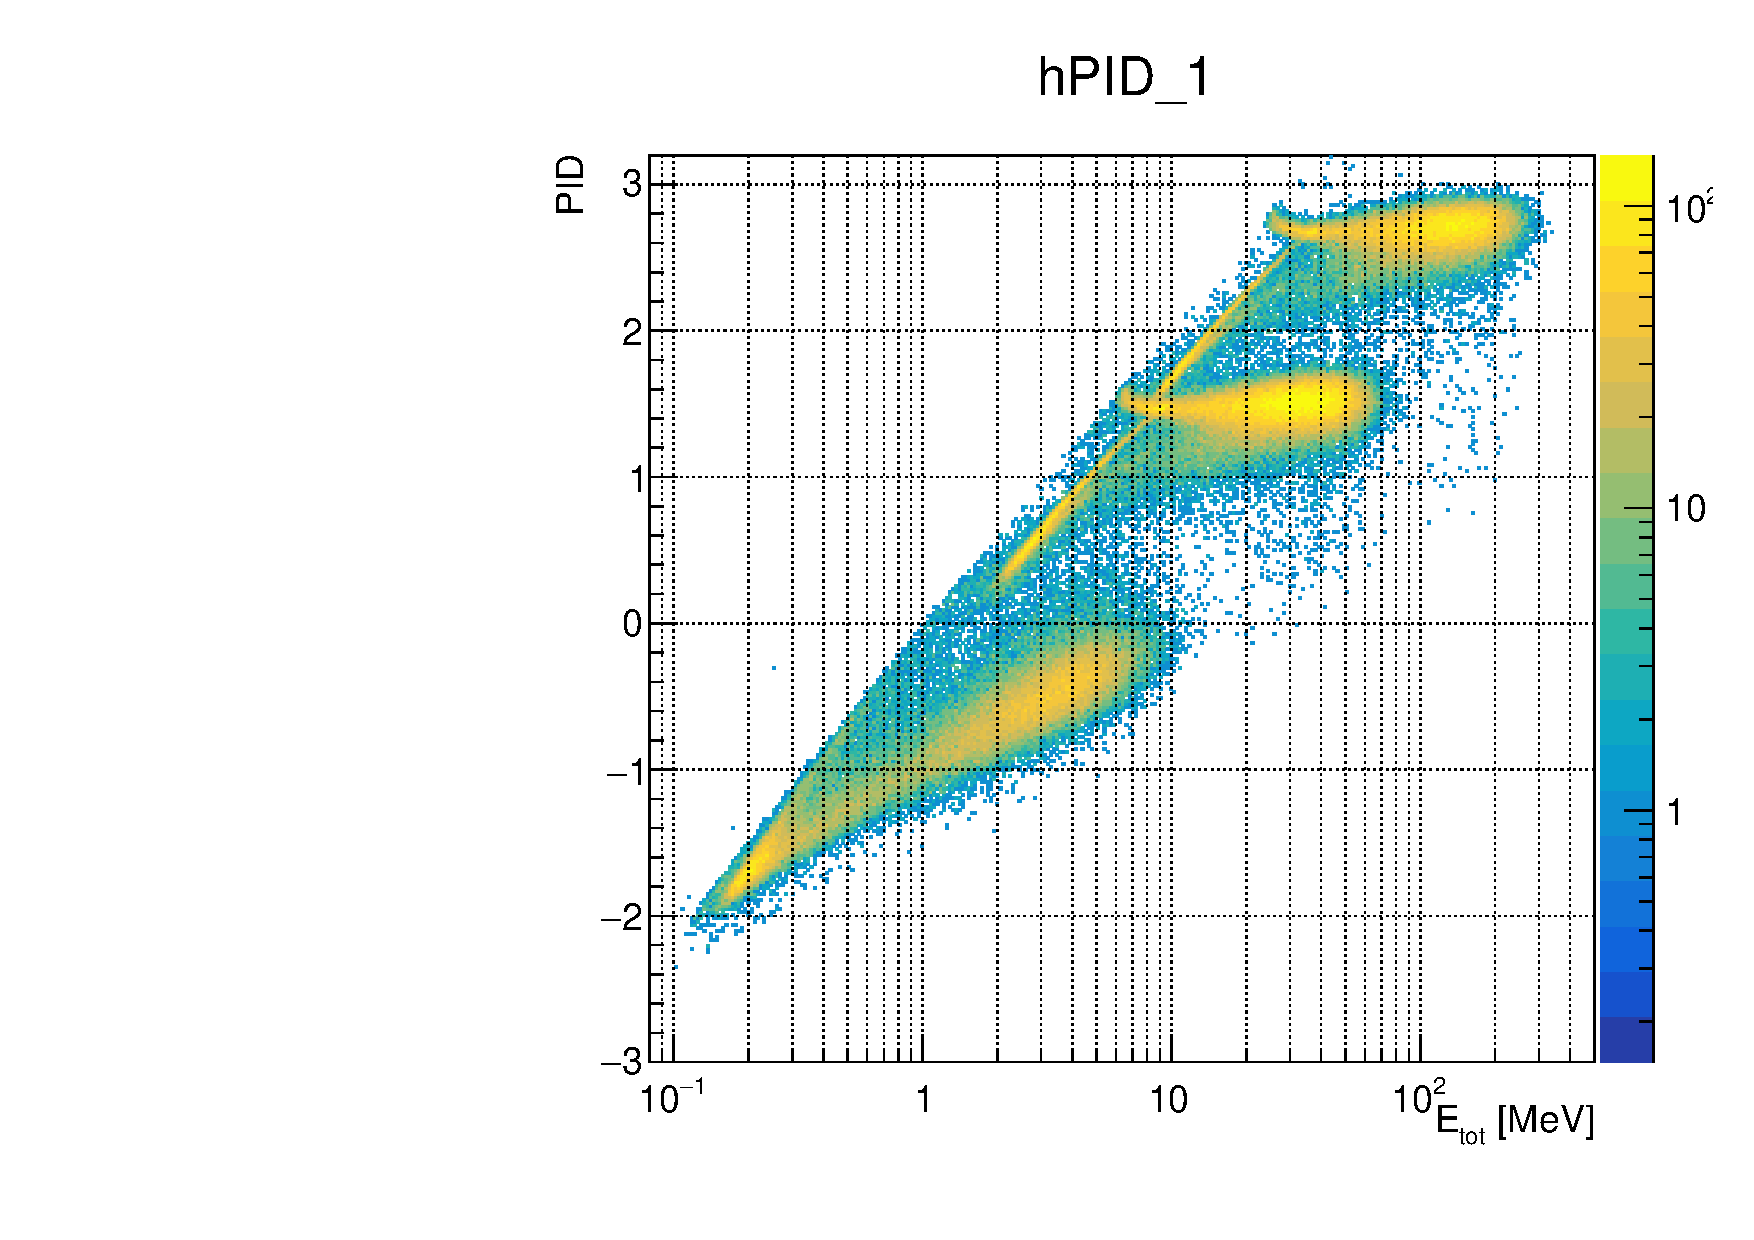
\includegraphics[width=1.0\textwidth]{/data1/home/rnicolai/LEM\_GDML\_upgrade/OUT/Output\_Geant4Simulation\_20230825/Analysis\_output/GDML\_file\_1/PID\_plots/gPID.pdf}
            \caption{PID, No Gaussian Smearing, Total Energy is the Energy reconstructed.}
        \end{figure}
        
            \end{frame}
            
            \begin{frame}
                \frametitle{PID No Calorimeter}
            
        \begin{figure}[h]
            \centering
            \includegraphics[width=1.0\textwidth]{/data1/home/rnicolai/LEM\_GDML\_upgrade/OUT/Output\_Geant4Simulation\_20230825/Analysis\_output/GDML\_file\_1/PID\_plots/gPID\_NoCalo.pdf}
            \caption{PID, No Gaussian Smearing, Total Energy is the Energy reconstructed, No Calorimeter.}
        \end{figure}
        
            \end{frame}
            
            \begin{frame}
                \frametitle{PID - Non Confinement Violation Factor - NOK}
            
        \begin{figure}[h]
            \centering
            \includegraphics[width=0.5\textwidth]{/data1/home/rnicolai/LEM\_GDML\_upgrade/OUT/Output\_Geant4Simulation\_20230825/Analysis\_output/GDML\_file\_1/PID\_plots/PID\_NCVF\_NOK.pdf}
            \caption{PID. Convined events but Measured energy is not equal to the MC energy.}
        \end{figure}
        
            \end{frame}
            
            \begin{frame}
                \frametitle{PID - Non Confinement Violation Factor - OK}
            
        \begin{figure}[h]
            \centering
            \includegraphics[width=0.5\textwidth]{/data1/home/rnicolai/LEM\_GDML\_upgrade/OUT/Output\_Geant4Simulation\_20230825/Analysis\_output/GDML\_file\_1/PID\_plots/PID\_NCVF\_OK.pdf}
            \caption{PID. Convined events and Measured energy is equal to the MC energy.}
        \end{figure}
        
            \end{frame}
            
            \begin{frame}
                \frametitle{PID - Non Confinement Violation Factor - NOK - No Calorimeter}
            
        \begin{figure}[h]
            \centering
            \includegraphics[width=0.5\textwidth]{/data1/home/rnicolai/LEM\_GDML\_upgrade/OUT/Output\_Geant4Simulation\_20230825/Analysis\_output/GDML\_file\_1/PID\_plots/PID\_NCVF\_NOK\_NoCalo.pdf}
            \caption{PID. Convined events but Measured energy is not equal to the MC energy. No Calorimeter.}
        \end{figure}
        
            \end{frame}
            
            \begin{frame}
                \frametitle{PID - Non Confinement Violation Factor - OK - No Calorimeter}
            
        \begin{figure}[h]
            \centering
            \includegraphics[width=0.5\textwidth]{/data1/home/rnicolai/LEM\_GDML\_upgrade/OUT/Output\_Geant4Simulation\_20230825/Analysis\_output/GDML\_file\_1/PID\_plots/PID\_NCVF\_OK\_NoCalo.pdf}
            \caption{PID. Convined events and Measured energy is equal to the MC energy. No Calorimeter.}
        \end{figure}
        
            \end{frame}
            
            \begin{frame}
                \frametitle{PID MC Energy}
            
        \begin{figure}[h]
            \centering
            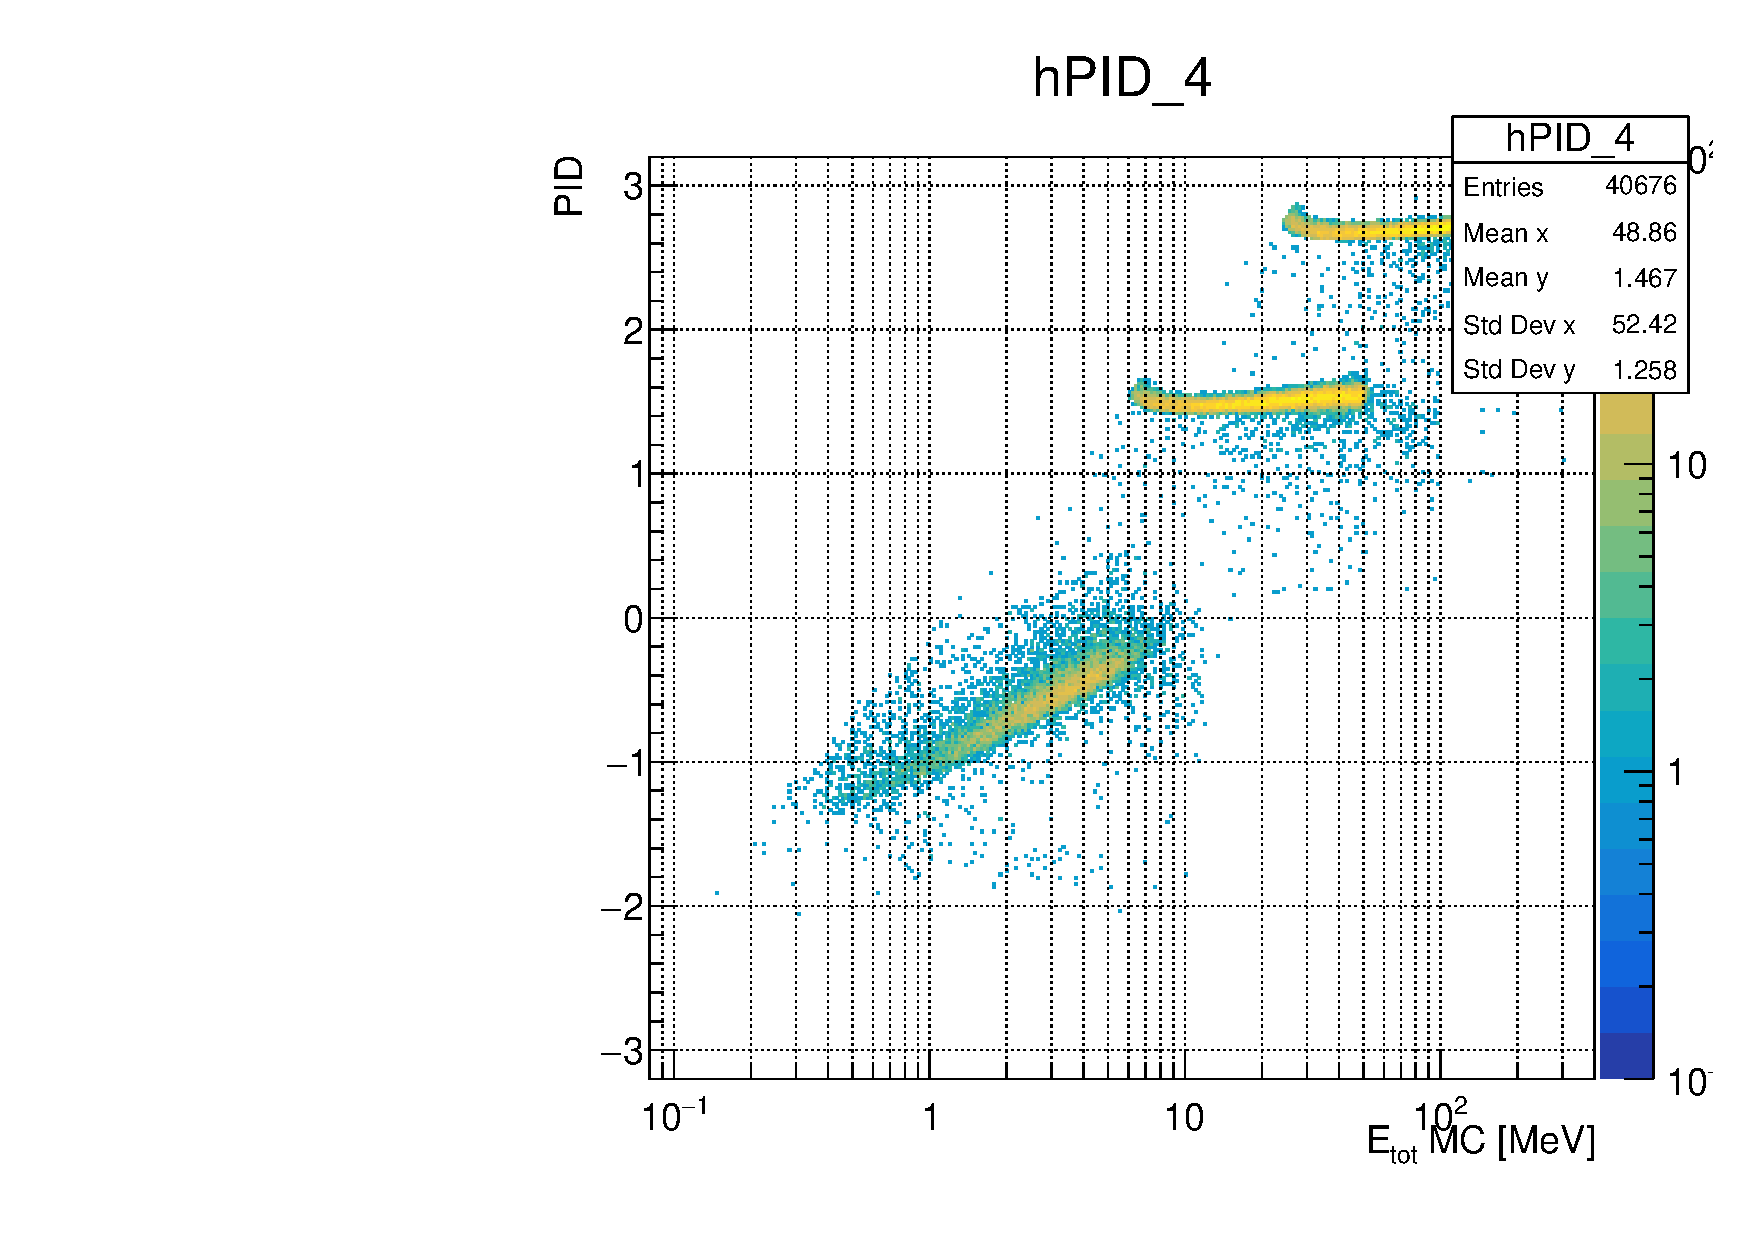
\includegraphics[width=1.0\textwidth]{/data1/home/rnicolai/LEM\_GDML\_upgrade/OUT/Output\_Geant4Simulation\_20230825/Analysis\_output/GDML\_file\_1/PID\_plots/PID2.pdf}
            \caption{PID, No Gaussian Smearing, Total Energy is the MC Energy.}
        \end{figure}
        
            \end{frame}
            
            \begin{frame}
                \frametitle{PID MC Energy No Calorimeter}
            
        \begin{figure}[h]
            \centering
            \includegraphics[width=1.0\textwidth]{/data1/home/rnicolai/LEM\_GDML\_upgrade/OUT/Output\_Geant4Simulation\_20230825/Analysis\_output/GDML\_file\_1/PID\_plots/gPID2\_NoCalo.pdf}
            \caption{PID, No Gaussian Smearing, Total Energy is the MC Energy, No Calorimeter.}
        \end{figure}
        
            \end{frame}
            
            \begin{frame}
                \frametitle{PID Gaussian Smearing}
            
        \begin{figure}[h]
            \centering
            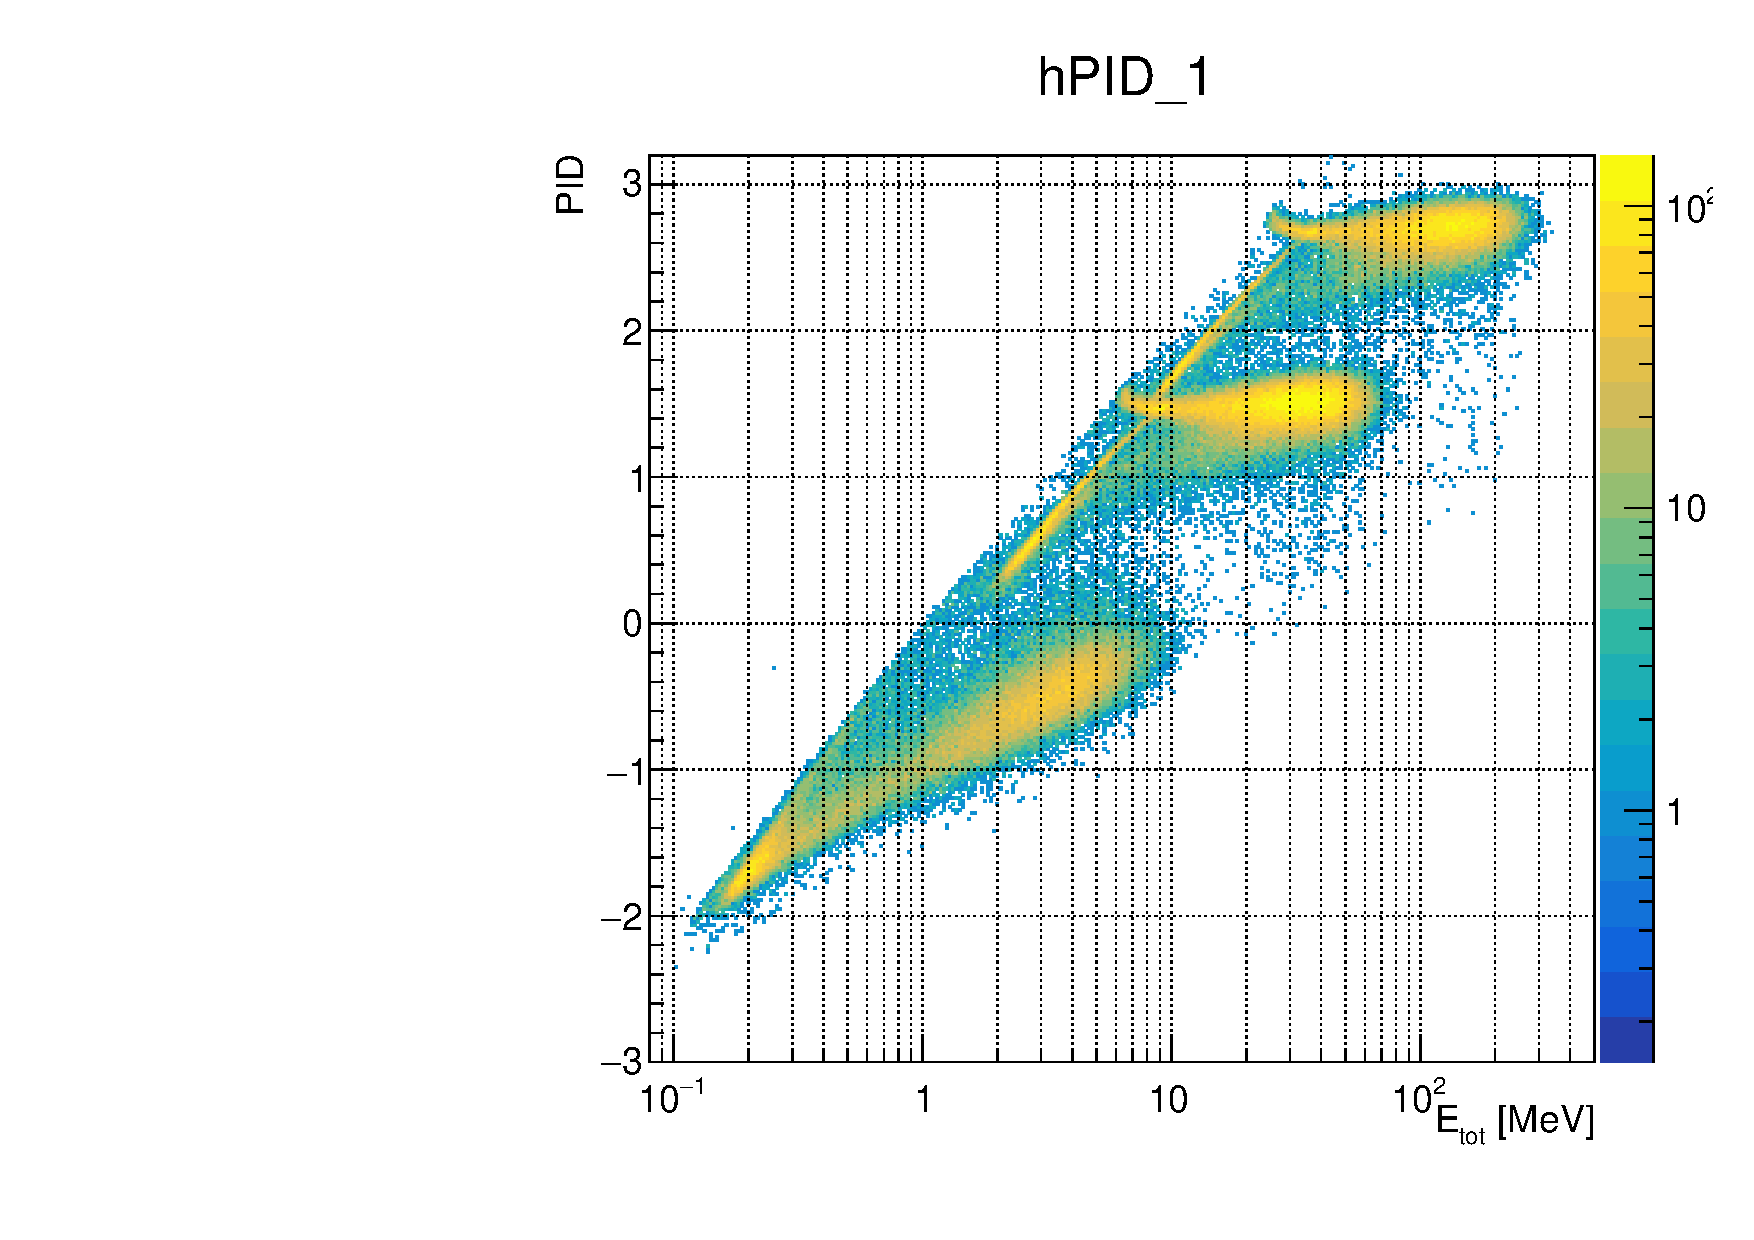
\includegraphics[width=1.0\textwidth]{/data1/home/rnicolai/LEM\_GDML\_upgrade/OUT/Output\_Geant4Simulation\_20230825/Analysis\_output/GDML\_file\_1/PID\_plots/gPID.pdf}
            \caption{PID, Gaussian Smearing, Total Energy is the Energy reconstructed.}
        \end{figure}
        
            \end{frame}
            
            \begin{frame}
                \frametitle{PID Gaussian Smearing No Calorimeter}
            
        \begin{figure}[h]
            \centering
            \includegraphics[width=1.0\textwidth]{/data1/home/rnicolai/LEM\_GDML\_upgrade/OUT/Output\_Geant4Simulation\_20230825/Analysis\_output/GDML\_file\_1/PID\_plots/gPID\_NoCalo.pdf}
            \caption{PID, Gaussian Smearing, Total Energy is the Energy reconstructed, No Calorimeter.}
        \end{figure}
        
            \end{frame}
            
            \begin{frame}
                \frametitle{PID MC Energy Gaussian Smearing}
            
        \begin{figure}[h]
            \centering
            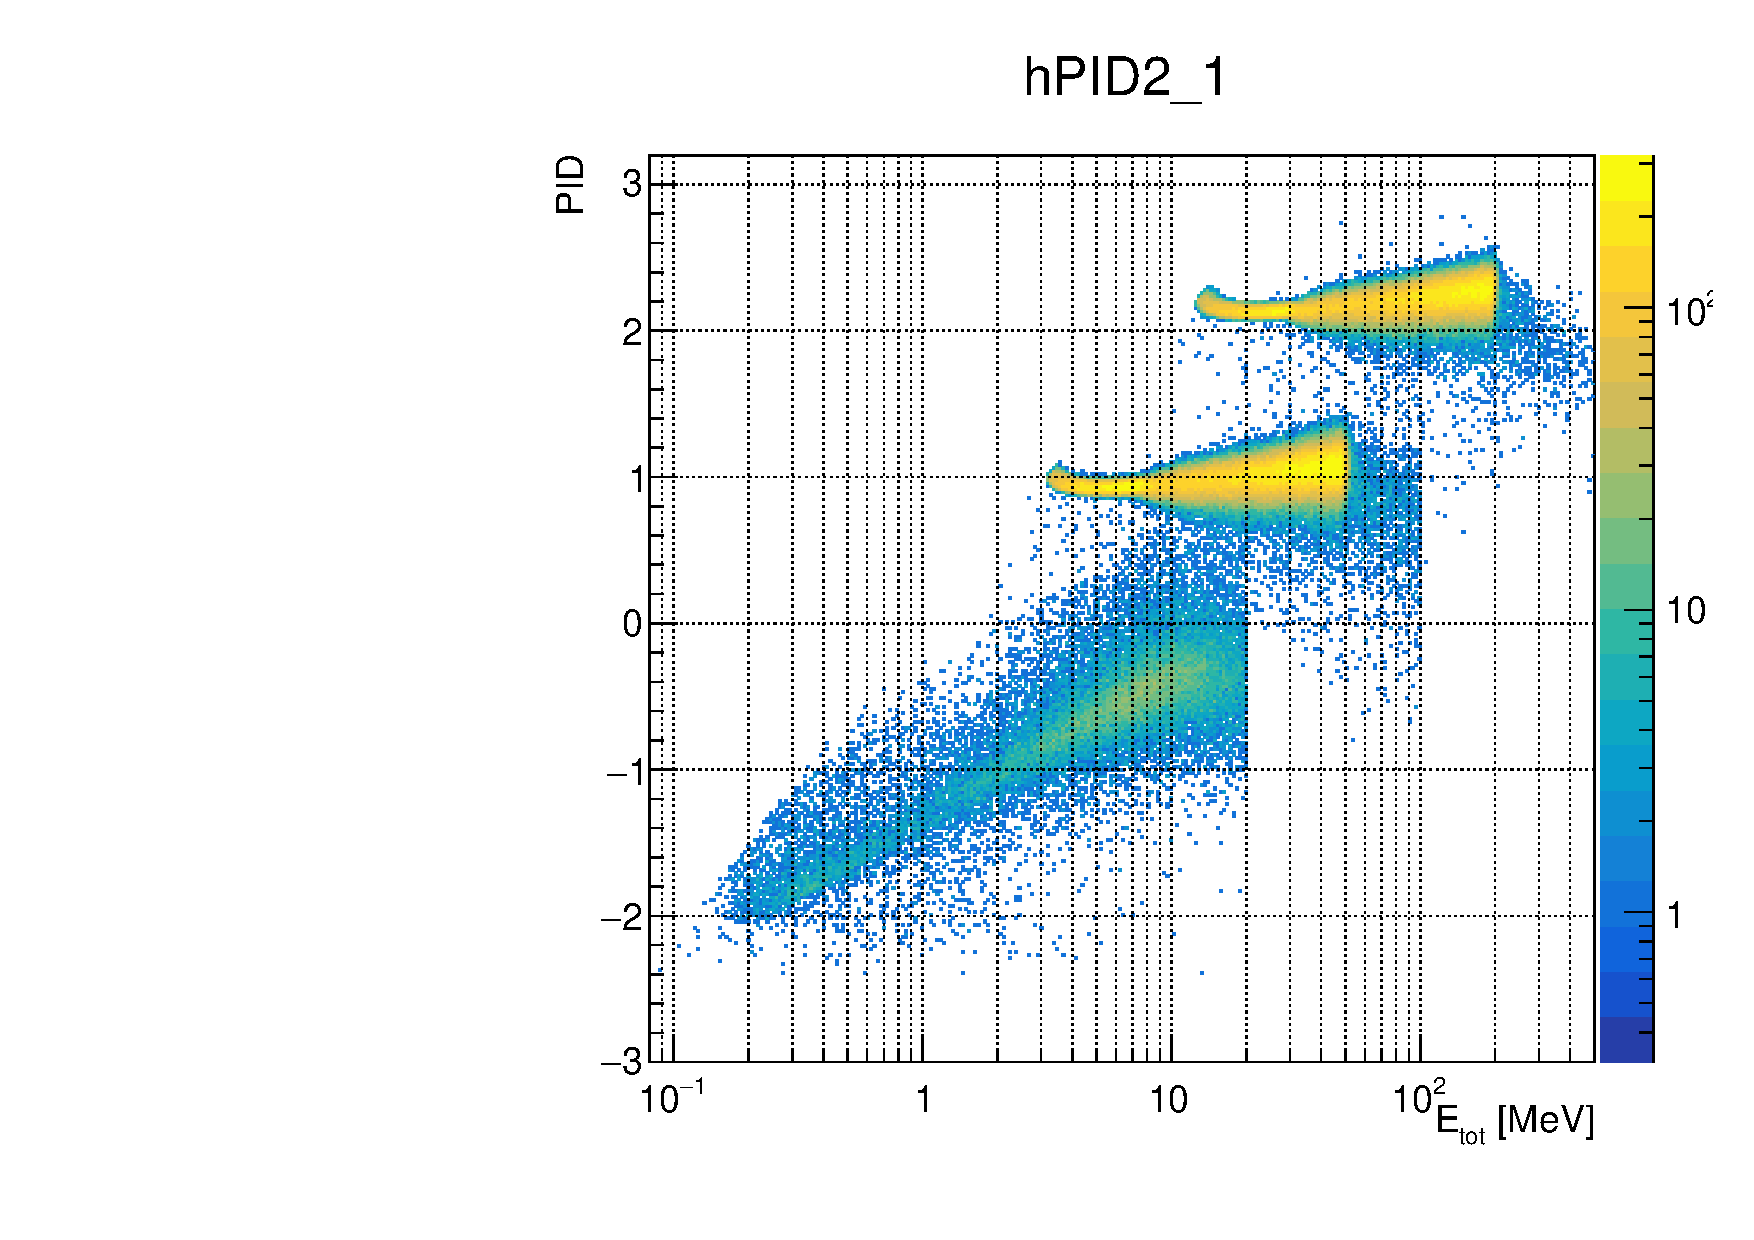
\includegraphics[width=1.0\textwidth]{/data1/home/rnicolai/LEM\_GDML\_upgrade/OUT/Output\_Geant4Simulation\_20230825/Analysis\_output/GDML\_file\_1/PID\_plots/gPID2.pdf}
            \caption{PID, Gaussian Smearing, Total Energy is the MC Energy.}
        \end{figure}
        
            \end{frame}
            
            \begin{frame}
                \frametitle{PID MC Energy Gaussian Smearing No Calorimeter}
            
        \begin{figure}[h]
            \centering
            \includegraphics[width=1.0\textwidth]{/data1/home/rnicolai/LEM\_GDML\_upgrade/OUT/Output\_Geant4Simulation\_20230825/Analysis\_output/GDML\_file\_1/PID\_plots/gPID2\_NoCalo.pdf}
            \caption{PID, Gaussian Smearing, Total Energy is the MC Energy, No Calorimeter.}
        \end{figure}
        
            \end{frame}
            
            \begin{frame}
                \frametitle{PID graphs}
            
        \begin{figure}[h]
            \centering
            \includegraphics[width=1.0\textwidth]{/data1/home/rnicolai/LEM\_GDML\_upgrade/OUT/Output\_Geant4Simulation\_20230825/Analysis\_output/GDML\_file\_1/PID\_plots/graph\_PID\_center.pdf}
            \caption{PID, Gaussian Smearing, Total Energy is the Energy reconstructed, No Calorimeter.}
        \end{figure}
        
            \end{frame}
            
            \begin{frame}
                \frametitle{MC quantities for e-\_t0}
            
        \begin{figure}[h]
            \centering
            \includegraphics[width=1.0\textwidth]{/data1/home/rnicolai/LEM\_GDML\_upgrade/OUT/Output\_Geant4Simulation\_20230825/Analysis\_output/GDML\_file\_1/Montecarlo\_e-\_t0.png}
            \caption{MC quantities}
        \end{figure}
        
        \begin{figure}[h]
            \centering
            \includegraphics[width=1.0\textwidth]{/data1/home/rnicolai/LEM\_GDML\_upgrade/OUT/Output\_Geant4Simulation\_20230825/Analysis\_output/GDML\_file\_1/Montecarlo\_e-\_t0.pdf}
            \caption{MC quantities}
        \end{figure}
        
            \end{frame}
            
            \begin{frame}
                \frametitle{Energies distribution for e-}
            
        \begin{figure}[h]
            \centering
            \includegraphics[width=1.0\textwidth]{/data1/home/rnicolai/LEM\_GDML\_upgrade/OUT/Output\_Geant4Simulation\_20230825/Analysis\_output/GDML\_file\_1/Energies\_e-\_t0.png}
            \caption{Detected energies}
        \end{figure}
        
        \begin{figure}[h]
            \centering
            \includegraphics[width=1.0\textwidth]{/data1/home/rnicolai/LEM\_GDML\_upgrade/OUT/Output\_Geant4Simulation\_20230825/Analysis\_output/GDML\_file\_1/Energies\_e-\_t0.pdf}
            \caption{Detected energies}
        \end{figure}
        
            \end{frame}
            
            \begin{frame}
                \frametitle{Angles distribution accepted for e-}
            
        \begin{figure}[h]
            \centering
            \includegraphics[width=1.0\textwidth]{/data1/home/rnicolai/LEM\_GDML\_upgrade/OUT/Output\_Geant4Simulation\_20230825/Analysis\_output/GDML\_file\_1/Angles\_e-\_t0.png}
            \caption{Angles distribution}
        \end{figure}
        
        \begin{figure}[h]
            \centering
            \includegraphics[width=1.0\textwidth]{/data1/home/rnicolai/LEM\_GDML\_upgrade/OUT/Output\_Geant4Simulation\_20230825/Analysis\_output/GDML\_file\_1/Angles\_e-\_t0.pdf}
            \caption{Angles distribution}
        \end{figure}
        
            \end{frame}
            
            \begin{frame}
                \frametitle{Angles distribution accepted for e-}
            
        \begin{figure}[h]
            \centering
            \includegraphics[width=1.0\textwidth]{/data1/home/rnicolai/LEM\_GDML\_upgrade/OUT/Output\_Geant4Simulation\_20230825/Analysis\_output/GDML\_file\_1/2DAngHistoFigure\_4\_e-\_t0\_e-\_t0.pdf}
            \caption{Angles distribution}
        \end{figure}
        
            \end{frame}
            
            \begin{frame}
                \frametitle{Angles distribution accepted for e-}
            
        \begin{figure}[h]
            \centering
            \includegraphics[width=1.0\textwidth]{/data1/home/rnicolai/LEM\_GDML\_upgrade/OUT/Output\_Geant4Simulation\_20230825/Analysis\_output/GDML\_file\_1/2DAngHistoFigure\_3\_e-\_t0\_e-\_t0.png}
            \caption{Angles distribution}
        \end{figure}
        
            \end{frame}
            
            \begin{frame}
                \frametitle{Angles distribution accepted for e-}
            
        \begin{figure}[h]
            \centering
            \includegraphics[width=1.0\textwidth]{/data1/home/rnicolai/LEM\_GDML\_upgrade/OUT/Output\_Geant4Simulation\_20230825/Analysis\_output/GDML\_file\_1/2DAngHistoFigure\_1\_e-\_t0\_e-\_t0.png}
            \caption{Angles distribution}
        \end{figure}
        
            \end{frame}
            
            \begin{frame}
                \frametitle{Angles distribution accepted for e-}
            
        \begin{figure}[h]
            \centering
            \includegraphics[width=1.0\textwidth]{/data1/home/rnicolai/LEM\_GDML\_upgrade/OUT/Output\_Geant4Simulation\_20230825/Analysis\_output/GDML\_file\_1/2DAngHistoFigure\_1\_e-\_t0\_e-\_t0.pdf}
            \caption{Angles distribution}
        \end{figure}
        
            \end{frame}
            
            \begin{frame}
                \frametitle{Angles distribution accepted for e-}
            
        \begin{figure}[h]
            \centering
            \includegraphics[width=1.0\textwidth]{/data1/home/rnicolai/LEM\_GDML\_upgrade/OUT/Output\_Geant4Simulation\_20230825/Analysis\_output/GDML\_file\_1/2DAngHistoFigure\_4\_e-\_t0\_e-\_t0.png}
            \caption{Angles distribution}
        \end{figure}
        
            \end{frame}
            
            \begin{frame}
                \frametitle{Angles distribution accepted for e-}
            
        \begin{figure}[h]
            \centering
            \includegraphics[width=1.0\textwidth]{/data1/home/rnicolai/LEM\_GDML\_upgrade/OUT/Output\_Geant4Simulation\_20230825/Analysis\_output/GDML\_file\_1/2DAngHistoFigure\_2\_e-\_t0\_e-\_t0.pdf}
            \caption{Angles distribution}
        \end{figure}
        
            \end{frame}
            
            \begin{frame}
                \frametitle{Angles distribution accepted for e-}
            
        \begin{figure}[h]
            \centering
            \includegraphics[width=1.0\textwidth]{/data1/home/rnicolai/LEM\_GDML\_upgrade/OUT/Output\_Geant4Simulation\_20230825/Analysis\_output/GDML\_file\_1/2DAngHistoFigure\_2\_e-\_t0\_e-\_t0.png}
            \caption{Angles distribution}
        \end{figure}
        
            \end{frame}
            
            \begin{frame}
                \frametitle{Angles distribution accepted for e-}
            
        \begin{figure}[h]
            \centering
            \includegraphics[width=1.0\textwidth]{/data1/home/rnicolai/LEM\_GDML\_upgrade/OUT/Output\_Geant4Simulation\_20230825/Analysis\_output/GDML\_file\_1/2DAngHistoFigure\_3\_e-\_t0\_e-\_t0.pdf}
            \caption{Angles distribution}
        \end{figure}
        
            \end{frame}
            
            \begin{frame}
                \frametitle{Angles distribution accepted for e-}
            
        \begin{figure}[h]
            \centering
            \includegraphics[width=1.0\textwidth]{/data1/home/rnicolai/LEM\_GDML\_upgrade/OUT/Output\_Geant4Simulation\_20230825/Analysis\_output/GDML\_file\_1/2DAngHistoFigure\_0\_e-\_t0\_e-\_t0.png}
            \caption{Angles distribution}
        \end{figure}
        
            \end{frame}
            
            \begin{frame}
                \frametitle{Angles distribution accepted for e-}
            
        \begin{figure}[h]
            \centering
            \includegraphics[width=1.0\textwidth]{/data1/home/rnicolai/LEM\_GDML\_upgrade/OUT/Output\_Geant4Simulation\_20230825/Analysis\_output/GDML\_file\_1/2DAngHistoFigure\_0\_e-\_t0\_e-\_t0.pdf}
            \caption{Angles distribution}
        \end{figure}
        
            \end{frame}
            
            \begin{frame}
                \frametitle{Generation Position distribution accepted for e-}
            
        \begin{figure}[h]
            \centering
            \includegraphics[width=1.0\textwidth]{/data1/home/rnicolai/LEM\_GDML\_upgrade/OUT/Output\_Geant4Simulation\_20230825/Analysis\_output/GDML\_file\_1/GenPosition\_3\_e-\_t0\_e-\_t0.pdf}
            \caption{Generation Position}
        \end{figure}
        
            \end{frame}
            
            \begin{frame}
                \frametitle{Generation Position distribution accepted for e-}
            
        \begin{figure}[h]
            \centering
            \includegraphics[width=1.0\textwidth]{/data1/home/rnicolai/LEM\_GDML\_upgrade/OUT/Output\_Geant4Simulation\_20230825/Analysis\_output/GDML\_file\_1/GenPosition\_1\_e-\_t0\_e-\_t0.png}
            \caption{Generation Position}
        \end{figure}
        
            \end{frame}
            
            \begin{frame}
                \frametitle{Generation Position distribution accepted for e-}
            
        \begin{figure}[h]
            \centering
            \includegraphics[width=1.0\textwidth]{/data1/home/rnicolai/LEM\_GDML\_upgrade/OUT/Output\_Geant4Simulation\_20230825/Analysis\_output/GDML\_file\_1/GenPosition\_3\_e-\_t0\_e-\_t0.png}
            \caption{Generation Position}
        \end{figure}
        
            \end{frame}
            
            \begin{frame}
                \frametitle{Generation Position distribution accepted for e-}
            
        \begin{figure}[h]
            \centering
            \includegraphics[width=1.0\textwidth]{/data1/home/rnicolai/LEM\_GDML\_upgrade/OUT/Output\_Geant4Simulation\_20230825/Analysis\_output/GDML\_file\_1/GenPosition\_4\_e-\_t0\_e-\_t0.png}
            \caption{Generation Position}
        \end{figure}
        
            \end{frame}
            
            \begin{frame}
                \frametitle{Generation Position distribution accepted for e-}
            
        \begin{figure}[h]
            \centering
            \includegraphics[width=1.0\textwidth]{/data1/home/rnicolai/LEM\_GDML\_upgrade/OUT/Output\_Geant4Simulation\_20230825/Analysis\_output/GDML\_file\_1/GenPosition\_4\_e-\_t0\_e-\_t0.pdf}
            \caption{Generation Position}
        \end{figure}
        
            \end{frame}
            
            \begin{frame}
                \frametitle{Generation Position distribution accepted for e-}
            
        \begin{figure}[h]
            \centering
            \includegraphics[width=1.0\textwidth]{/data1/home/rnicolai/LEM\_GDML\_upgrade/OUT/Output\_Geant4Simulation\_20230825/Analysis\_output/GDML\_file\_1/GenPosition\_1\_e-\_t0\_e-\_t0.pdf}
            \caption{Generation Position}
        \end{figure}
        
            \end{frame}
            
            \begin{frame}
                \frametitle{Generation Position distribution accepted for e-}
            
        \begin{figure}[h]
            \centering
            \includegraphics[width=1.0\textwidth]{/data1/home/rnicolai/LEM\_GDML\_upgrade/OUT/Output\_Geant4Simulation\_20230825/Analysis\_output/GDML\_file\_1/GenPosition\_2\_e-\_t0\_e-\_t0.png}
            \caption{Generation Position}
        \end{figure}
        
            \end{frame}
            
            \begin{frame}
                \frametitle{Generation Position distribution accepted for e-}
            
        \begin{figure}[h]
            \centering
            \includegraphics[width=1.0\textwidth]{/data1/home/rnicolai/LEM\_GDML\_upgrade/OUT/Output\_Geant4Simulation\_20230825/Analysis\_output/GDML\_file\_1/GenPosition\_2\_e-\_t0\_e-\_t0.pdf}
            \caption{Generation Position}
        \end{figure}
        
            \end{frame}
            
            \begin{frame}
                \frametitle{Generation Position distribution accepted for e-}
            
        \begin{figure}[h]
            \centering
            \includegraphics[width=1.0\textwidth]{/data1/home/rnicolai/LEM\_GDML\_upgrade/OUT/Output\_Geant4Simulation\_20230825/Analysis\_output/GDML\_file\_1/GenPosition\_0\_e-\_t0\_e-\_t0.pdf}
            \caption{Generation Position}
        \end{figure}
        
            \end{frame}
            
            \begin{frame}
                \frametitle{Generation Position distribution accepted for e-}
            
        \begin{figure}[h]
            \centering
            \includegraphics[width=1.0\textwidth]{/data1/home/rnicolai/LEM\_GDML\_upgrade/OUT/Output\_Geant4Simulation\_20230825/Analysis\_output/GDML\_file\_1/GenPosition\_0\_e-\_t0\_e-\_t0.png}
            \caption{Generation Position}
        \end{figure}
        
            \end{frame}
            
            \begin{frame}
                \frametitle{Geometric factors for e-}
            
            \end{frame}
            
            \begin{frame}
                \frametitle{Geometric factors for e-}
            
            \end{frame}
            
            \begin{frame}
                \frametitle{MC quantities for proton\_t0}
            
        \begin{figure}[h]
            \centering
            \includegraphics[width=1.0\textwidth]{/data1/home/rnicolai/LEM\_GDML\_upgrade/OUT/Output\_Geant4Simulation\_20230825/Analysis\_output/GDML\_file\_1/Montecarlo\_proton\_t0.pdf}
            \caption{MC quantities}
        \end{figure}
        
        \begin{figure}[h]
            \centering
            \includegraphics[width=1.0\textwidth]{/data1/home/rnicolai/LEM\_GDML\_upgrade/OUT/Output\_Geant4Simulation\_20230825/Analysis\_output/GDML\_file\_1/Montecarlo\_proton\_t0.png}
            \caption{MC quantities}
        \end{figure}
        
            \end{frame}
            
            \begin{frame}
                \frametitle{Energies distribution for proton}
            
        \begin{figure}[h]
            \centering
            \includegraphics[width=1.0\textwidth]{/data1/home/rnicolai/LEM\_GDML\_upgrade/OUT/Output\_Geant4Simulation\_20230825/Analysis\_output/GDML\_file\_1/Energies\_proton\_t0.png}
            \caption{Detected energies}
        \end{figure}
        
        \begin{figure}[h]
            \centering
            \includegraphics[width=1.0\textwidth]{/data1/home/rnicolai/LEM\_GDML\_upgrade/OUT/Output\_Geant4Simulation\_20230825/Analysis\_output/GDML\_file\_1/Energies\_proton\_t0.pdf}
            \caption{Detected energies}
        \end{figure}
        
            \end{frame}
            
            \begin{frame}
                \frametitle{Angles distribution accepted for proton}
            
        \begin{figure}[h]
            \centering
            \includegraphics[width=1.0\textwidth]{/data1/home/rnicolai/LEM\_GDML\_upgrade/OUT/Output\_Geant4Simulation\_20230825/Analysis\_output/GDML\_file\_1/Angles\_proton\_t0.png}
            \caption{Angles distribution}
        \end{figure}
        
        \begin{figure}[h]
            \centering
            \includegraphics[width=1.0\textwidth]{/data1/home/rnicolai/LEM\_GDML\_upgrade/OUT/Output\_Geant4Simulation\_20230825/Analysis\_output/GDML\_file\_1/Angles\_proton\_t0.pdf}
            \caption{Angles distribution}
        \end{figure}
        
            \end{frame}
            
            \begin{frame}
                \frametitle{Angles distribution accepted for proton}
            
        \begin{figure}[h]
            \centering
            \includegraphics[width=1.0\textwidth]{/data1/home/rnicolai/LEM\_GDML\_upgrade/OUT/Output\_Geant4Simulation\_20230825/Analysis\_output/GDML\_file\_1/2DAngHistoFigure\_1\_proton\_t0\_proton\_t0.png}
            \caption{Angles distribution}
        \end{figure}
        
            \end{frame}
            
            \begin{frame}
                \frametitle{Angles distribution accepted for proton}
            
        \begin{figure}[h]
            \centering
            \includegraphics[width=1.0\textwidth]{/data1/home/rnicolai/LEM\_GDML\_upgrade/OUT/Output\_Geant4Simulation\_20230825/Analysis\_output/GDML\_file\_1/2DAngHistoFigure\_3\_proton\_t0\_proton\_t0.png}
            \caption{Angles distribution}
        \end{figure}
        
            \end{frame}
            
            \begin{frame}
                \frametitle{Angles distribution accepted for proton}
            
        \begin{figure}[h]
            \centering
            \includegraphics[width=1.0\textwidth]{/data1/home/rnicolai/LEM\_GDML\_upgrade/OUT/Output\_Geant4Simulation\_20230825/Analysis\_output/GDML\_file\_1/2DAngHistoFigure\_2\_proton\_t0\_proton\_t0.pdf}
            \caption{Angles distribution}
        \end{figure}
        
            \end{frame}
            
            \begin{frame}
                \frametitle{Angles distribution accepted for proton}
            
        \begin{figure}[h]
            \centering
            \includegraphics[width=1.0\textwidth]{/data1/home/rnicolai/LEM\_GDML\_upgrade/OUT/Output\_Geant4Simulation\_20230825/Analysis\_output/GDML\_file\_1/2DAngHistoFigure\_1\_proton\_t0\_proton\_t0.pdf}
            \caption{Angles distribution}
        \end{figure}
        
            \end{frame}
            
            \begin{frame}
                \frametitle{Angles distribution accepted for proton}
            
        \begin{figure}[h]
            \centering
            \includegraphics[width=1.0\textwidth]{/data1/home/rnicolai/LEM\_GDML\_upgrade/OUT/Output\_Geant4Simulation\_20230825/Analysis\_output/GDML\_file\_1/2DAngHistoFigure\_4\_proton\_t0\_proton\_t0.png}
            \caption{Angles distribution}
        \end{figure}
        
            \end{frame}
            
            \begin{frame}
                \frametitle{Angles distribution accepted for proton}
            
        \begin{figure}[h]
            \centering
            \includegraphics[width=1.0\textwidth]{/data1/home/rnicolai/LEM\_GDML\_upgrade/OUT/Output\_Geant4Simulation\_20230825/Analysis\_output/GDML\_file\_1/2DAngHistoFigure\_4\_proton\_t0\_proton\_t0.pdf}
            \caption{Angles distribution}
        \end{figure}
        
            \end{frame}
            
            \begin{frame}
                \frametitle{Angles distribution accepted for proton}
            
        \begin{figure}[h]
            \centering
            \includegraphics[width=1.0\textwidth]{/data1/home/rnicolai/LEM\_GDML\_upgrade/OUT/Output\_Geant4Simulation\_20230825/Analysis\_output/GDML\_file\_1/2DAngHistoFigure\_3\_proton\_t0\_proton\_t0.pdf}
            \caption{Angles distribution}
        \end{figure}
        
            \end{frame}
            
            \begin{frame}
                \frametitle{Angles distribution accepted for proton}
            
        \begin{figure}[h]
            \centering
            \includegraphics[width=1.0\textwidth]{/data1/home/rnicolai/LEM\_GDML\_upgrade/OUT/Output\_Geant4Simulation\_20230825/Analysis\_output/GDML\_file\_1/2DAngHistoFigure\_0\_proton\_t0\_proton\_t0.pdf}
            \caption{Angles distribution}
        \end{figure}
        
            \end{frame}
            
            \begin{frame}
                \frametitle{Angles distribution accepted for proton}
            
        \begin{figure}[h]
            \centering
            \includegraphics[width=1.0\textwidth]{/data1/home/rnicolai/LEM\_GDML\_upgrade/OUT/Output\_Geant4Simulation\_20230825/Analysis\_output/GDML\_file\_1/2DAngHistoFigure\_2\_proton\_t0\_proton\_t0.png}
            \caption{Angles distribution}
        \end{figure}
        
            \end{frame}
            
            \begin{frame}
                \frametitle{Angles distribution accepted for proton}
            
        \begin{figure}[h]
            \centering
            \includegraphics[width=1.0\textwidth]{/data1/home/rnicolai/LEM\_GDML\_upgrade/OUT/Output\_Geant4Simulation\_20230825/Analysis\_output/GDML\_file\_1/2DAngHistoFigure\_0\_proton\_t0\_proton\_t0.png}
            \caption{Angles distribution}
        \end{figure}
        
            \end{frame}
            
            \begin{frame}
                \frametitle{Generation Position distribution accepted for proton}
            
        \begin{figure}[h]
            \centering
            \includegraphics[width=1.0\textwidth]{/data1/home/rnicolai/LEM\_GDML\_upgrade/OUT/Output\_Geant4Simulation\_20230825/Analysis\_output/GDML\_file\_1/GenPosition\_1\_proton\_t0\_proton\_t0.png}
            \caption{Generation Position}
        \end{figure}
        
            \end{frame}
            
            \begin{frame}
                \frametitle{Generation Position distribution accepted for proton}
            
        \begin{figure}[h]
            \centering
            \includegraphics[width=1.0\textwidth]{/data1/home/rnicolai/LEM\_GDML\_upgrade/OUT/Output\_Geant4Simulation\_20230825/Analysis\_output/GDML\_file\_1/GenPosition\_3\_proton\_t0\_proton\_t0.png}
            \caption{Generation Position}
        \end{figure}
        
            \end{frame}
            
            \begin{frame}
                \frametitle{Generation Position distribution accepted for proton}
            
        \begin{figure}[h]
            \centering
            \includegraphics[width=1.0\textwidth]{/data1/home/rnicolai/LEM\_GDML\_upgrade/OUT/Output\_Geant4Simulation\_20230825/Analysis\_output/GDML\_file\_1/GenPosition\_4\_proton\_t0\_proton\_t0.png}
            \caption{Generation Position}
        \end{figure}
        
            \end{frame}
            
            \begin{frame}
                \frametitle{Generation Position distribution accepted for proton}
            
        \begin{figure}[h]
            \centering
            \includegraphics[width=1.0\textwidth]{/data1/home/rnicolai/LEM\_GDML\_upgrade/OUT/Output\_Geant4Simulation\_20230825/Analysis\_output/GDML\_file\_1/GenPosition\_0\_proton\_t0\_proton\_t0.pdf}
            \caption{Generation Position}
        \end{figure}
        
            \end{frame}
            
            \begin{frame}
                \frametitle{Generation Position distribution accepted for proton}
            
        \begin{figure}[h]
            \centering
            \includegraphics[width=1.0\textwidth]{/data1/home/rnicolai/LEM\_GDML\_upgrade/OUT/Output\_Geant4Simulation\_20230825/Analysis\_output/GDML\_file\_1/GenPosition\_2\_proton\_t0\_proton\_t0.pdf}
            \caption{Generation Position}
        \end{figure}
        
            \end{frame}
            
            \begin{frame}
                \frametitle{Generation Position distribution accepted for proton}
            
        \begin{figure}[h]
            \centering
            \includegraphics[width=1.0\textwidth]{/data1/home/rnicolai/LEM\_GDML\_upgrade/OUT/Output\_Geant4Simulation\_20230825/Analysis\_output/GDML\_file\_1/GenPosition\_3\_proton\_t0\_proton\_t0.pdf}
            \caption{Generation Position}
        \end{figure}
        
            \end{frame}
            
            \begin{frame}
                \frametitle{Generation Position distribution accepted for proton}
            
        \begin{figure}[h]
            \centering
            \includegraphics[width=1.0\textwidth]{/data1/home/rnicolai/LEM\_GDML\_upgrade/OUT/Output\_Geant4Simulation\_20230825/Analysis\_output/GDML\_file\_1/GenPosition\_2\_proton\_t0\_proton\_t0.png}
            \caption{Generation Position}
        \end{figure}
        
            \end{frame}
            
            \begin{frame}
                \frametitle{Generation Position distribution accepted for proton}
            
        \begin{figure}[h]
            \centering
            \includegraphics[width=1.0\textwidth]{/data1/home/rnicolai/LEM\_GDML\_upgrade/OUT/Output\_Geant4Simulation\_20230825/Analysis\_output/GDML\_file\_1/GenPosition\_1\_proton\_t0\_proton\_t0.pdf}
            \caption{Generation Position}
        \end{figure}
        
            \end{frame}
            
            \begin{frame}
                \frametitle{Generation Position distribution accepted for proton}
            
        \begin{figure}[h]
            \centering
            \includegraphics[width=1.0\textwidth]{/data1/home/rnicolai/LEM\_GDML\_upgrade/OUT/Output\_Geant4Simulation\_20230825/Analysis\_output/GDML\_file\_1/GenPosition\_0\_proton\_t0\_proton\_t0.png}
            \caption{Generation Position}
        \end{figure}
        
            \end{frame}
            
            \begin{frame}
                \frametitle{Generation Position distribution accepted for proton}
            
        \begin{figure}[h]
            \centering
            \includegraphics[width=1.0\textwidth]{/data1/home/rnicolai/LEM\_GDML\_upgrade/OUT/Output\_Geant4Simulation\_20230825/Analysis\_output/GDML\_file\_1/GenPosition\_4\_proton\_t0\_proton\_t0.pdf}
            \caption{Generation Position}
        \end{figure}
        
            \end{frame}
            
            \begin{frame}
                \frametitle{Geometric factors for proton}
            
            \end{frame}
            
            \begin{frame}
                \frametitle{Geometric factors for proton}
            
            \end{frame}
            
            \begin{frame}
                \frametitle{MC quantities for alpha\_t0}
            
        \begin{figure}[h]
            \centering
            \includegraphics[width=1.0\textwidth]{/data1/home/rnicolai/LEM\_GDML\_upgrade/OUT/Output\_Geant4Simulation\_20230825/Analysis\_output/GDML\_file\_1/Montecarlo\_alpha\_t0.pdf}
            \caption{MC quantities}
        \end{figure}
        
        \begin{figure}[h]
            \centering
            \includegraphics[width=1.0\textwidth]{/data1/home/rnicolai/LEM\_GDML\_upgrade/OUT/Output\_Geant4Simulation\_20230825/Analysis\_output/GDML\_file\_1/Montecarlo\_alpha\_t0.png}
            \caption{MC quantities}
        \end{figure}
        
            \end{frame}
            
            \begin{frame}
                \frametitle{Energies distribution for alpha}
            
        \begin{figure}[h]
            \centering
            \includegraphics[width=1.0\textwidth]{/data1/home/rnicolai/LEM\_GDML\_upgrade/OUT/Output\_Geant4Simulation\_20230825/Analysis\_output/GDML\_file\_1/Energies\_alpha\_t0.pdf}
            \caption{Detected energies}
        \end{figure}
        
        \begin{figure}[h]
            \centering
            \includegraphics[width=1.0\textwidth]{/data1/home/rnicolai/LEM\_GDML\_upgrade/OUT/Output\_Geant4Simulation\_20230825/Analysis\_output/GDML\_file\_1/Energies\_alpha\_t0.png}
            \caption{Detected energies}
        \end{figure}
        
            \end{frame}
            
            \begin{frame}
                \frametitle{Angles distribution accepted for alpha}
            
        \begin{figure}[h]
            \centering
            \includegraphics[width=1.0\textwidth]{/data1/home/rnicolai/LEM\_GDML\_upgrade/OUT/Output\_Geant4Simulation\_20230825/Analysis\_output/GDML\_file\_1/Angles\_alpha\_t0.pdf}
            \caption{Angles distribution}
        \end{figure}
        
        \begin{figure}[h]
            \centering
            \includegraphics[width=1.0\textwidth]{/data1/home/rnicolai/LEM\_GDML\_upgrade/OUT/Output\_Geant4Simulation\_20230825/Analysis\_output/GDML\_file\_1/Angles\_alpha\_t0.png}
            \caption{Angles distribution}
        \end{figure}
        
            \end{frame}
            
            \begin{frame}
                \frametitle{Angles distribution accepted for alpha}
            
        \begin{figure}[h]
            \centering
            \includegraphics[width=1.0\textwidth]{/data1/home/rnicolai/LEM\_GDML\_upgrade/OUT/Output\_Geant4Simulation\_20230825/Analysis\_output/GDML\_file\_1/2DAngHistoFigure\_2\_alpha\_t0\_alpha\_t0.png}
            \caption{Angles distribution}
        \end{figure}
        
            \end{frame}
            
            \begin{frame}
                \frametitle{Angles distribution accepted for alpha}
            
        \begin{figure}[h]
            \centering
            \includegraphics[width=1.0\textwidth]{/data1/home/rnicolai/LEM\_GDML\_upgrade/OUT/Output\_Geant4Simulation\_20230825/Analysis\_output/GDML\_file\_1/2DAngHistoFigure\_1\_alpha\_t0\_alpha\_t0.png}
            \caption{Angles distribution}
        \end{figure}
        
            \end{frame}
            
            \begin{frame}
                \frametitle{Angles distribution accepted for alpha}
            
        \begin{figure}[h]
            \centering
            \includegraphics[width=1.0\textwidth]{/data1/home/rnicolai/LEM\_GDML\_upgrade/OUT/Output\_Geant4Simulation\_20230825/Analysis\_output/GDML\_file\_1/2DAngHistoFigure\_3\_alpha\_t0\_alpha\_t0.png}
            \caption{Angles distribution}
        \end{figure}
        
            \end{frame}
            
            \begin{frame}
                \frametitle{Angles distribution accepted for alpha}
            
        \begin{figure}[h]
            \centering
            \includegraphics[width=1.0\textwidth]{/data1/home/rnicolai/LEM\_GDML\_upgrade/OUT/Output\_Geant4Simulation\_20230825/Analysis\_output/GDML\_file\_1/2DAngHistoFigure\_4\_alpha\_t0\_alpha\_t0.png}
            \caption{Angles distribution}
        \end{figure}
        
            \end{frame}
            
            \begin{frame}
                \frametitle{Angles distribution accepted for alpha}
            
        \begin{figure}[h]
            \centering
            \includegraphics[width=1.0\textwidth]{/data1/home/rnicolai/LEM\_GDML\_upgrade/OUT/Output\_Geant4Simulation\_20230825/Analysis\_output/GDML\_file\_1/2DAngHistoFigure\_2\_alpha\_t0\_alpha\_t0.pdf}
            \caption{Angles distribution}
        \end{figure}
        
            \end{frame}
            
            \begin{frame}
                \frametitle{Angles distribution accepted for alpha}
            
        \begin{figure}[h]
            \centering
            \includegraphics[width=1.0\textwidth]{/data1/home/rnicolai/LEM\_GDML\_upgrade/OUT/Output\_Geant4Simulation\_20230825/Analysis\_output/GDML\_file\_1/2DAngHistoFigure\_4\_alpha\_t0\_alpha\_t0.pdf}
            \caption{Angles distribution}
        \end{figure}
        
            \end{frame}
            
            \begin{frame}
                \frametitle{Angles distribution accepted for alpha}
            
        \begin{figure}[h]
            \centering
            \includegraphics[width=1.0\textwidth]{/data1/home/rnicolai/LEM\_GDML\_upgrade/OUT/Output\_Geant4Simulation\_20230825/Analysis\_output/GDML\_file\_1/2DAngHistoFigure\_0\_alpha\_t0\_alpha\_t0.pdf}
            \caption{Angles distribution}
        \end{figure}
        
            \end{frame}
            
            \begin{frame}
                \frametitle{Angles distribution accepted for alpha}
            
        \begin{figure}[h]
            \centering
            \includegraphics[width=1.0\textwidth]{/data1/home/rnicolai/LEM\_GDML\_upgrade/OUT/Output\_Geant4Simulation\_20230825/Analysis\_output/GDML\_file\_1/2DAngHistoFigure\_1\_alpha\_t0\_alpha\_t0.pdf}
            \caption{Angles distribution}
        \end{figure}
        
            \end{frame}
            
            \begin{frame}
                \frametitle{Angles distribution accepted for alpha}
            
        \begin{figure}[h]
            \centering
            \includegraphics[width=1.0\textwidth]{/data1/home/rnicolai/LEM\_GDML\_upgrade/OUT/Output\_Geant4Simulation\_20230825/Analysis\_output/GDML\_file\_1/2DAngHistoFigure\_3\_alpha\_t0\_alpha\_t0.pdf}
            \caption{Angles distribution}
        \end{figure}
        
            \end{frame}
            
            \begin{frame}
                \frametitle{Angles distribution accepted for alpha}
            
        \begin{figure}[h]
            \centering
            \includegraphics[width=1.0\textwidth]{/data1/home/rnicolai/LEM\_GDML\_upgrade/OUT/Output\_Geant4Simulation\_20230825/Analysis\_output/GDML\_file\_1/2DAngHistoFigure\_0\_alpha\_t0\_alpha\_t0.png}
            \caption{Angles distribution}
        \end{figure}
        
            \end{frame}
            
            \begin{frame}
                \frametitle{Generation Position distribution accepted for alpha}
            
        \begin{figure}[h]
            \centering
            \includegraphics[width=1.0\textwidth]{/data1/home/rnicolai/LEM\_GDML\_upgrade/OUT/Output\_Geant4Simulation\_20230825/Analysis\_output/GDML\_file\_1/GenPosition\_3\_alpha\_t0\_alpha\_t0.png}
            \caption{Generation Position}
        \end{figure}
        
            \end{frame}
            
            \begin{frame}
                \frametitle{Generation Position distribution accepted for alpha}
            
        \begin{figure}[h]
            \centering
            \includegraphics[width=1.0\textwidth]{/data1/home/rnicolai/LEM\_GDML\_upgrade/OUT/Output\_Geant4Simulation\_20230825/Analysis\_output/GDML\_file\_1/GenPosition\_0\_alpha\_t0\_alpha\_t0.png}
            \caption{Generation Position}
        \end{figure}
        
            \end{frame}
            
            \begin{frame}
                \frametitle{Generation Position distribution accepted for alpha}
            
        \begin{figure}[h]
            \centering
            \includegraphics[width=1.0\textwidth]{/data1/home/rnicolai/LEM\_GDML\_upgrade/OUT/Output\_Geant4Simulation\_20230825/Analysis\_output/GDML\_file\_1/GenPosition\_1\_alpha\_t0\_alpha\_t0.png}
            \caption{Generation Position}
        \end{figure}
        
            \end{frame}
            
            \begin{frame}
                \frametitle{Generation Position distribution accepted for alpha}
            
        \begin{figure}[h]
            \centering
            \includegraphics[width=1.0\textwidth]{/data1/home/rnicolai/LEM\_GDML\_upgrade/OUT/Output\_Geant4Simulation\_20230825/Analysis\_output/GDML\_file\_1/GenPosition\_2\_alpha\_t0\_alpha\_t0.png}
            \caption{Generation Position}
        \end{figure}
        
            \end{frame}
            
            \begin{frame}
                \frametitle{Generation Position distribution accepted for alpha}
            
        \begin{figure}[h]
            \centering
            \includegraphics[width=1.0\textwidth]{/data1/home/rnicolai/LEM\_GDML\_upgrade/OUT/Output\_Geant4Simulation\_20230825/Analysis\_output/GDML\_file\_1/GenPosition\_2\_alpha\_t0\_alpha\_t0.pdf}
            \caption{Generation Position}
        \end{figure}
        
            \end{frame}
            
            \begin{frame}
                \frametitle{Generation Position distribution accepted for alpha}
            
        \begin{figure}[h]
            \centering
            \includegraphics[width=1.0\textwidth]{/data1/home/rnicolai/LEM\_GDML\_upgrade/OUT/Output\_Geant4Simulation\_20230825/Analysis\_output/GDML\_file\_1/GenPosition\_4\_alpha\_t0\_alpha\_t0.pdf}
            \caption{Generation Position}
        \end{figure}
        
            \end{frame}
            
            \begin{frame}
                \frametitle{Generation Position distribution accepted for alpha}
            
        \begin{figure}[h]
            \centering
            \includegraphics[width=1.0\textwidth]{/data1/home/rnicolai/LEM\_GDML\_upgrade/OUT/Output\_Geant4Simulation\_20230825/Analysis\_output/GDML\_file\_1/GenPosition\_4\_alpha\_t0\_alpha\_t0.png}
            \caption{Generation Position}
        \end{figure}
        
            \end{frame}
            
            \begin{frame}
                \frametitle{Generation Position distribution accepted for alpha}
            
        \begin{figure}[h]
            \centering
            \includegraphics[width=1.0\textwidth]{/data1/home/rnicolai/LEM\_GDML\_upgrade/OUT/Output\_Geant4Simulation\_20230825/Analysis\_output/GDML\_file\_1/GenPosition\_3\_alpha\_t0\_alpha\_t0.pdf}
            \caption{Generation Position}
        \end{figure}
        
            \end{frame}
            
            \begin{frame}
                \frametitle{Generation Position distribution accepted for alpha}
            
        \begin{figure}[h]
            \centering
            \includegraphics[width=1.0\textwidth]{/data1/home/rnicolai/LEM\_GDML\_upgrade/OUT/Output\_Geant4Simulation\_20230825/Analysis\_output/GDML\_file\_1/GenPosition\_0\_alpha\_t0\_alpha\_t0.pdf}
            \caption{Generation Position}
        \end{figure}
        
            \end{frame}
            
            \begin{frame}
                \frametitle{Generation Position distribution accepted for alpha}
            
        \begin{figure}[h]
            \centering
            \includegraphics[width=1.0\textwidth]{/data1/home/rnicolai/LEM\_GDML\_upgrade/OUT/Output\_Geant4Simulation\_20230825/Analysis\_output/GDML\_file\_1/GenPosition\_1\_alpha\_t0\_alpha\_t0.pdf}
            \caption{Generation Position}
        \end{figure}
        
            \end{frame}
            
            \begin{frame}
                \frametitle{Geometric factors for alpha}
            
            \end{frame}
            
            \begin{frame}
                \frametitle{Geometric factors for alpha}
            
            \end{frame}
            
            \begin{frame}
                \frametitle{Geometric factors for all particles}
            
            \end{frame}
            
        \end{document}
        